\documentclass[aspectratio=169,10pt,compress]{beamer}

\useoutertheme{split}
\useinnertheme{rounded}
\usecolortheme{whale}
\usecolortheme{orchid}
\setbeamertemplate{blocks}[rounded]
\setbeamertemplate{navigation symbols}{}
\setbeamertemplate{page number in head/foot}[totalframenumber]
% split footline shows "i / N" (frame number / total frames) on every frame

\usepackage[T1]{fontenc}
\usepackage{lmodern}
\usepackage{listings}
\usepackage{xcolor}
\usepackage{booktabs}
\usepackage{array}
\usepackage{tikz}
\usetikzlibrary{positioning,arrows.meta,calc}

\newcolumntype{L}[1]{>{\raggedright\arraybackslash}p{#1}}

\definecolor{codebg}{RGB}{245,245,245}
\definecolor{codecomment}{RGB}{110,110,110}
\definecolor{gitred}{RGB}{240,80,50}
\definecolor{gitblue}{RGB}{40,90,160}
\definecolor{gitgreen}{RGB}{40,130,70}

\lstset{
  language=bash,
  basicstyle=\ttfamily\footnotesize,
  backgroundcolor=\color{codebg},
  commentstyle=\color{codecomment}\itshape,
  keywordstyle=\color{gitred}\bfseries,
  morekeywords={git},
  frame=single,
  rulecolor=\color{gray!40},
  columns=fullflexible,
  keepspaces=true,
  showstringspaces=false,
  breaklines=true,
  xleftmargin=4pt,
  xrightmargin=4pt,
  aboveskip=4pt,
  belowskip=4pt
}

\newcommand{\cmd}[1]{\texttt{\color{gitred}#1}}

\tikzset{
  commit/.style={circle, draw=gitblue, fill=gitblue!15, thick, minimum size=7mm,
                 inner sep=0pt, font=\scriptsize\ttfamily},
  newcommit/.style={commit, draw=gitred, fill=gitred!15},
  edge/.style={-{Stealth[length=2mm]}, thick, gray!70},
  lbl/.style={font=\scriptsize\bfseries, text=gitred},
  obj/.style={draw, rounded corners, thick, minimum width=2.4cm, minimum height=0.9cm,
              align=center, font=\scriptsize},
  ref/.style={draw, thick, fill=gitred!15, draw=gitred, minimum height=0.6cm,
              font=\scriptsize\ttfamily}
}

\title{Git for Seniors}
\subtitle{Internals, Automation and Scale}
\author[Bingol]{Haluk O. Bingol}

\institute[FCIS]{
    Faculty of Computer and Information Sciences\\
    Yeditepe University
}
\date{}

\begin{document}

% ~~~~~~~~~~~~~~~~~~~~~~~~~~~~~~~~~~~~~~ V
\begin{frame}[t,fragile]
  \titlepage
\end{frame}
% ~~~~~~~~~~~~~~~~~~~~~~~~~~~~~~~~~~~~~~ A

% ~~~~~~~~~~~~~~~~~~~~~~~~~~~~~~~~~~~~~~ V
\begin{frame}[t,fragile] \frametitle{Outline}
  \begin{columns}[T]
    \begin{column}{0.5\textwidth}
      \tableofcontents[sections={1-6}]
    \end{column}
    \begin{column}{0.5\textwidth}
      \tableofcontents[sections={7-12}]
    \end{column}
  \end{columns}
\end{frame}
% ~~~~~~~~~~~~~~~~~~~~~~~~~~~~~~~~~~~~~~ A

% ~~~~~~~~~~~~~~~~~~~~~~~~~~~~~~~~~~~~~~ V
\begin{frame}[t,fragile] \frametitle{Where we are}
  \textbf{You already know} (junior level):
  \begin{itemize}
    \item forks, pull requests, branching strategies
    \item rebase, \cmd{rebase -i}, fixup commits, stash, \cmd{add -p}
    \item \cmd{reset} modes, \cmd{revert}, the reflog, \cmd{log -S}, \cmd{blame}, tags
  \end{itemize}

  \vspace{0.5em}
  \textbf{This lecture:} becoming the person who \emph{fixes} the repository
  \begin{itemize}
    \item how Git stores data, so that no command feels like magic
    \item finding bugs, automating checks, and cleaning up history
    \item working with large repositories and securing your work
  \end{itemize}

  \vspace{0.5em}
  \begin{block}{Goal}
    Predict what any Git command will do before you run it.
  \end{block}
\end{frame}
% ~~~~~~~~~~~~~~~~~~~~~~~~~~~~~~~~~~~~~~ A

% ~~~~~~~~~~~~~~~~~~~~~~~~~~~~~~~~~~~~~~ V
\section[Internals]{Git Internals}
% ~~~~~~~~~~~~~~~~~~~~~~~~~~~~~~~~~~~~~~ A

% ~~~~~~~~~~~~~~~~~~~~~~~~~~~~~~~~~~~~~~ V
\begin{frame}[t,fragile] \frametitle{The object model}
  Git is a \textbf{content-addressed key--value store}. Every object is named by the hash of its content.

  \vspace{0.3em}
  \begin{center}
  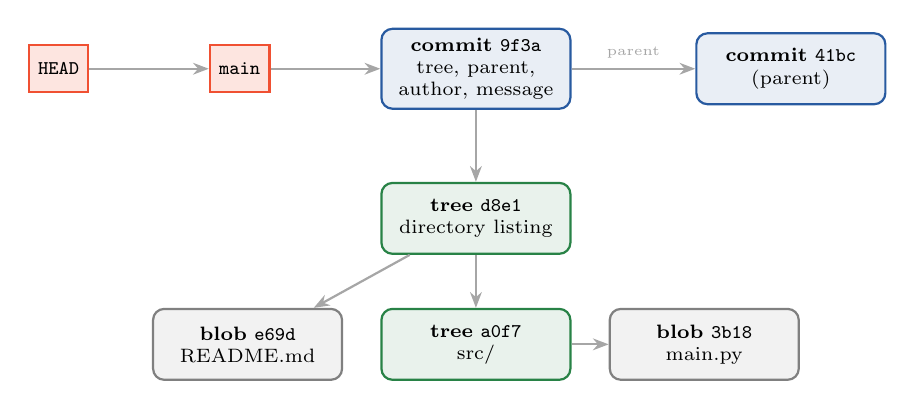
\begin{tikzpicture}
    \node[ref] (head) at (0,0) {HEAD};
    \node[ref] (main) at (2.3,0) {main};
    \node[obj, draw=gitblue, fill=gitblue!10] (c2) at (5.3,0) {\textbf{commit} \texttt{9f3a}\\ tree, parent,\\ author, message};
    \node[obj, draw=gitblue, fill=gitblue!10] (c1) at (9.3,0) {\textbf{commit} \texttt{41bc}\\ (parent)};
    \node[obj, draw=gitgreen, fill=gitgreen!10] (t) at (5.3,-1.9) {\textbf{tree} \texttt{d8e1}\\ directory listing};
    \node[obj, draw=gray, fill=gray!10] (b1) at (2.4,-3.5) {\textbf{blob} \texttt{e69d}\\ README.md};
    \node[obj, draw=gitgreen, fill=gitgreen!10] (t2) at (5.3,-3.5) {\textbf{tree} \texttt{a0f7}\\ src/};
    \node[obj, draw=gray, fill=gray!10] (b2) at (8.2,-3.5) {\textbf{blob} \texttt{3b18}\\ main.py};
    \draw[edge] (head) -- (main);
    \draw[edge] (main) -- (c2);
    \draw[edge] (c2) -- node[above, font=\tiny]{parent} (c1);
    \draw[edge] (c2) -- (t);
    \draw[edge] (t) -- (b1);
    \draw[edge] (t) -- (t2);
    \draw[edge] (t2) -- (b2);
  \end{tikzpicture}
  \end{center}

  \small
  \textbf{Blob:} file contents (no name).
  \textbf{Tree:} names $\rightarrow$ blobs/trees.
  \textbf{Commit:} a tree + parents + metadata.
  \textbf{Branch:} a movable pointer to a commit.
\end{frame}
% ~~~~~~~~~~~~~~~~~~~~~~~~~~~~~~~~~~~~~~ A

% ~~~~~~~~~~~~~~~~~~~~~~~~~~~~~~~~~~~~~~ V
\begin{frame}[t,fragile] \frametitle{Exploring with plumbing commands}
\begin{lstlisting}
git cat-file -t HEAD              # commit
git cat-file -p HEAD              # tree d8e1..., parent 41bc..., author, message
git cat-file -p 'HEAD^{tree}'     # 100644 blob e69d... README.md
                                  # 040000 tree a0f7... src
git ls-tree -r HEAD               # every file in the snapshot

echo "hello" | git hash-object --stdin    # same content -> same hash, always
cat .git/HEAD                     # ref: refs/heads/main
cat .git/refs/heads/main          # 9f3a...  (just a hash in a text file!)
\end{lstlisting}

  \begin{block}{The big idea}
    A branch is a tiny file holding one commit hash. Creating a branch costs almost nothing,
    and \cmd{reset}, \cmd{rebase} and the reflog are just ways of moving that pointer.
  \end{block}
  \vspace{-0.3em}
  {\scriptsize Note: refs may be packed into \texttt{.git/packed-refs}; \cmd{git rev-parse main} always works.}
\end{frame}
% ~~~~~~~~~~~~~~~~~~~~~~~~~~~~~~~~~~~~~~ A

% ~~~~~~~~~~~~~~~~~~~~~~~~~~~~~~~~~~~~~~ V
\section[Merging]{Advanced Merging}
% ~~~~~~~~~~~~~~~~~~~~~~~~~~~~~~~~~~~~~~ A

% ~~~~~~~~~~~~~~~~~~~~~~~~~~~~~~~~~~~~~~ V
\begin{frame}[t,fragile] \frametitle{Three-way merge and the merge base}
  \begin{columns}[T]
    \begin{column}{0.45\textwidth}
      \centering
      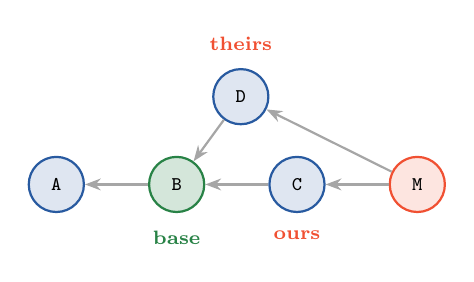
\begin{tikzpicture}[node distance=8mm]
        \node[commit] (a) {A};
        \node[commit, draw=gitgreen, fill=gitgreen!20, right=of a] (b) {B};
        \node[commit, right=of b] (c) {C};
        \node[commit, above right=6mm and 3mm of b] (d) {D};
        \node[newcommit, right=of c] (m) {M};
        \draw[edge] (b) -- (a); \draw[edge] (c) -- (b);
        \draw[edge] (d) -- (b);
        \draw[edge] (m) -- (c); \draw[edge] (m) -- (d);
        \node[lbl, text=gitgreen, below=1mm of b] {base};
        \node[lbl, below=1mm of c] {ours};
        \node[lbl, above=1mm of d] {theirs};
      \end{tikzpicture}
    \end{column}
    \begin{column}{0.52\textwidth}
      \small
      Git compares \textbf{three} versions of each file:
      \begin{itemize}
        \item \textbf{base:} the common ancestor
        \item \textbf{ours:} the current branch
        \item \textbf{theirs:} the branch being merged
      \end{itemize}
      A side that differs from base wins. If \emph{both} differ in the same place: conflict.
    \end{column}
  \end{columns}

\begin{lstlisting}
git merge-base main feature       # find B
git config --global merge.conflictStyle zdiff3   # show base in conflicts
git checkout --ours file.txt      # take our side of a conflicted file
git checkout --theirs file.txt    # take their side
\end{lstlisting}
\end{frame}
% ~~~~~~~~~~~~~~~~~~~~~~~~~~~~~~~~~~~~~~ A

% ~~~~~~~~~~~~~~~~~~~~~~~~~~~~~~~~~~~~~~ V
\begin{frame}[t,fragile] \frametitle{Merge strategies and \texttt{rerere}}
  \textbf{Strategies} (\cmd{git merge -s <strategy>})
  \begin{itemize}
    \item \texttt{ort}: the default since Git 2.34; handles renames well
    \item \texttt{ours}: record a merge but keep our tree unchanged
          (e.g.\ mark an old branch as ``merged'' without taking its changes)
    \item \texttt{-X ours} / \texttt{-X theirs}: an \emph{option} to \texttt{ort} that
          auto-resolves only conflicting hunks. Not the same as \texttt{-s ours}!
  \end{itemize}

  \vspace{0.3em}
  \textbf{rerere: ``reuse recorded resolution''}
\begin{lstlisting}
git config --global rerere.enabled true
\end{lstlisting}
  \small
  Git remembers how you resolved each conflict. When the same conflict appears
  again (repeated rebases, long-lived branches), it resolves it for you.

  \begin{block}{Tools}
    \cmd{git mergetool} opens a visual 3-way merge (VS Code, Meld, KDiff3, vimdiff).
  \end{block}
\end{frame}
% ~~~~~~~~~~~~~~~~~~~~~~~~~~~~~~~~~~~~~~ A

% ~~~~~~~~~~~~~~~~~~~~~~~~~~~~~~~~~~~~~~ V
\section[Bisect]{Debugging with Bisect}
% ~~~~~~~~~~~~~~~~~~~~~~~~~~~~~~~~~~~~~~ A

% ~~~~~~~~~~~~~~~~~~~~~~~~~~~~~~~~~~~~~~ V
\begin{frame}[t,fragile] \frametitle{\texttt{git bisect}: binary search for bugs}
  Tests passed at \texttt{v2.0}; 500 commits later they fail. Which commit broke them?

  \begin{center}
  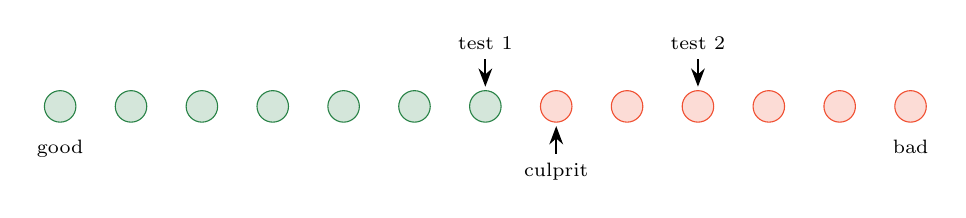
\begin{tikzpicture}[x=0.9cm]
    \foreach \i in {0,...,6}
      \node[circle, draw=gitgreen, fill=gitgreen!20, minimum size=4mm, inner sep=0] at (\i,0) {};
    \foreach \i in {7,...,12}
      \node[circle, draw=gitred, fill=gitred!20, minimum size=4mm, inner sep=0] at (\i,0) {};
    \node[font=\scriptsize, below=3mm] at (0,0) {good};
    \node[font=\scriptsize, below=3mm] at (12,0) {bad};
    \draw[-{Stealth}, thick] (6,0.6) -- (6,0.25); \node[font=\scriptsize, above] at (6,0.6) {test 1};
    \draw[-{Stealth}, thick] (9,0.6) -- (9,0.25); \node[font=\scriptsize, above] at (9,0.6) {test 2};
    \draw[-{Stealth}, thick] (7,-0.6) -- (7,-0.25); \node[font=\scriptsize, below] at (7,-0.6) {culprit};
  \end{tikzpicture}
  \end{center}

\begin{lstlisting}
git bisect start
git bisect bad                    # current commit is broken
git bisect good v2.0              # this one worked
# Git checks out a commit in the middle. Test it, then:
git bisect good                   # or: git bisect bad
# ...repeat about log2(500) = 9 times...
git bisect reset                  # return to where you started
\end{lstlisting}
\end{frame}
% ~~~~~~~~~~~~~~~~~~~~~~~~~~~~~~~~~~~~~~ A

% ~~~~~~~~~~~~~~~~~~~~~~~~~~~~~~~~~~~~~~ V
\begin{frame}[t,fragile] \frametitle{Automated bisect}
  Let a script do the testing. Its exit code tells Git the answer:

  \begin{columns}[T]
    \begin{column}{0.55\textwidth}
\begin{lstlisting}
# test.sh
#!/bin/sh
make || exit 125     # can't build: skip
./run_tests          # 0 = good, 1 = bad
\end{lstlisting}
\begin{lstlisting}
git bisect start HEAD v2.0
git bisect run ./test.sh
# ...
# 7c1d9e2 is the first bad commit
git bisect reset
\end{lstlisting}
    \end{column}
    \begin{column}{0.42\textwidth}
      \small
      \begin{tabular}{@{}ll@{}}
        \toprule
        \textbf{Exit code} & \textbf{Meaning} \\
        \midrule
        0 & good \\
        1--124, 126, 127 & bad \\
        125 & skip this commit \\
        \bottomrule
      \end{tabular}

      \vspace{1em}
      \begin{block}{Why it matters}
        Minutes instead of hours, and it works best when every commit builds
        (another reason for atomic commits).
      \end{block}
    \end{column}
  \end{columns}
\end{frame}
% ~~~~~~~~~~~~~~~~~~~~~~~~~~~~~~~~~~~~~~ A

% ~~~~~~~~~~~~~~~~~~~~~~~~~~~~~~~~~~~~~~ V
\section[Backport]{Cherry-pick and Backporting}
% ~~~~~~~~~~~~~~~~~~~~~~~~~~~~~~~~~~~~~~ A

% ~~~~~~~~~~~~~~~~~~~~~~~~~~~~~~~~~~~~~~ V
\begin{frame}[t,fragile] \frametitle{Cherry-pick: copy one commit elsewhere}
  A security fix landed on \texttt{main}; version 1.x users need it too.

  \begin{center}
  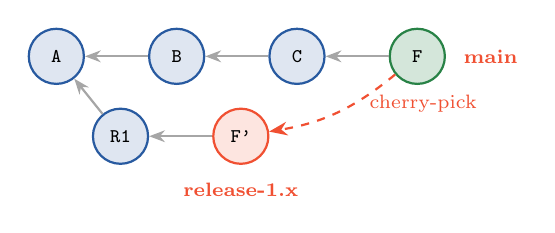
\begin{tikzpicture}[node distance=8mm]
    \node[commit] (a) {A};
    \node[commit, right=of a] (b) {B};
    \node[commit, right=of b] (c) {C};
    \node[commit, draw=gitgreen, fill=gitgreen!20, right=of c] (f) {F};
    \node[commit, below right=5mm and 3mm of a] (r1) {R1};
    \node[newcommit, right=of r1] (fp) {F'};
    \draw[edge] (b) -- (a); \draw[edge] (c) -- (b); \draw[edge] (f) -- (c);
    \draw[edge] (r1) -- (a); \draw[edge] (fp) -- (r1);
    \draw[-{Stealth}, dashed, gitred, thick] (f) to[bend left=15] node[right=2pt, font=\scriptsize, text=gitred, pos=0.35]{cherry-pick} (fp);
    \node[lbl, right=1mm of f] {main};
    \node[lbl, below=1mm of fp] {release-1.x};
  \end{tikzpicture}
  \end{center}

\begin{lstlisting}
git switch release-1.x
git cherry-pick -x a1b2c3d        # -x adds "(cherry picked from commit ...)"
git cherry-pick a1b2c3d^..f6e5d4c # a range of commits
# conflict? fix it, git add, then:
git cherry-pick --continue        # or --abort
\end{lstlisting}
  \small \textbf{Caution:} \texttt{F'} is a \emph{new} commit with a different hash.
  Prefer fixing on the oldest branch and merging forward when you can.
\end{frame}
% ~~~~~~~~~~~~~~~~~~~~~~~~~~~~~~~~~~~~~~ A

% ~~~~~~~~~~~~~~~~~~~~~~~~~~~~~~~~~~~~~~ V
\section[CI/CD]{Hooks and CI/CD}
% ~~~~~~~~~~~~~~~~~~~~~~~~~~~~~~~~~~~~~~ A

% ~~~~~~~~~~~~~~~~~~~~~~~~~~~~~~~~~~~~~~ V
\begin{frame}[t,fragile] \frametitle{Git hooks}
  Hooks are scripts Git runs at certain moments. They live in \texttt{.git/hooks/}.

  \begin{columns}[T]
    \begin{column}{0.5\textwidth}
      \small
      \begin{tabular}{@{}ll@{}}
        \toprule
        \textbf{Hook} & \textbf{Typical use} \\
        \midrule
        \texttt{pre-commit} & lint, format, tests \\
        \texttt{commit-msg} & enforce message style \\
        \texttt{pre-push} & run the full test suite \\
        \texttt{pre-receive} & server: reject bad pushes \\
        \bottomrule
      \end{tabular}
    \end{column}
    \begin{column}{0.47\textwidth}
\begin{lstlisting}
# .git/hooks/pre-commit
#!/bin/sh
python -m flake8 . || exit 1
# non-zero exit = commit refused
\end{lstlisting}
    \end{column}
  \end{columns}

  \vspace{0.3em}
  \textbf{Sharing hooks with the team:} \texttt{.git/hooks} is not versioned, so use the
  \texttt{pre-commit} framework or \cmd{git config core.hooksPath .githooks}
\begin{lstlisting}[language={}]
# .pre-commit-config.yaml         then run:  pre-commit install
repos:
  - repo: https://github.com/psf/black
    rev: 24.8.0
    hooks: [{id: black}]
\end{lstlisting}
\end{frame}
% ~~~~~~~~~~~~~~~~~~~~~~~~~~~~~~~~~~~~~~ A

% ~~~~~~~~~~~~~~~~~~~~~~~~~~~~~~~~~~~~~~ V
\begin{frame}[t,fragile] \frametitle{CI/CD: checks on every push}
  \begin{columns}[T]
    \begin{column}{0.52\textwidth}
\begin{lstlisting}[language={}]
# .github/workflows/test.yml
name: tests
on: [push, pull_request]
jobs:
  test:
    runs-on: ubuntu-latest
    steps:
      - uses: actions/checkout@v4
      - uses: actions/setup-python@v5
        with: {python-version: "3.12"}
      - run: pip install -r requirements.txt
      - run: pytest
\end{lstlisting}
    \end{column}
    \begin{column}{0.45\textwidth}
      \textbf{Branch protection on \texttt{main}}
      \begin{itemize}\small
        \item require a pull request
        \item require $\ge$ 1 approving review
        \item require status checks (CI) to pass
        \item block force pushes and deletion
      \end{itemize}
      \vspace{0.3em}
      \begin{block}{Hooks vs.\ CI}
        \small Hooks are fast, local and skippable (\texttt{--no-verify}).
        CI is the check nobody can skip.
      \end{block}
    \end{column}
  \end{columns}
\end{frame}
% ~~~~~~~~~~~~~~~~~~~~~~~~~~~~~~~~~~~~~~ A

% ~~~~~~~~~~~~~~~~~~~~~~~~~~~~~~~~~~~~~~ V
\section[Rewrite]{Rewriting History at Scale}
% ~~~~~~~~~~~~~~~~~~~~~~~~~~~~~~~~~~~~~~ A

% ~~~~~~~~~~~~~~~~~~~~~~~~~~~~~~~~~~~~~~ V
\begin{frame}[t,fragile] \frametitle{Removing a leaked secret from all history}
  Someone committed \texttt{.env} with an API key three weeks ago.
  Deleting it in a new commit is \textbf{not enough}: it is still in every old snapshot.

  \vspace{0.3em}
  \begin{enumerate}\small
    \item \textbf{Rotate the key first.} Assume it is already compromised.
    \item Rewrite history with \texttt{git filter-repo} (\cmd{pip install git-filter-repo}):
  \end{enumerate}
\begin{lstlisting}
git clone --mirror https://github.com/team/app.git   # work on a fresh copy
cd app.git
git filter-repo --path .env --invert-paths          # drop the file everywhere
git filter-repo --replace-text ../patterns.txt      # or scrub strings
git push --force --mirror
\end{lstlisting}
  \begin{enumerate}\small
    \setcounter{enumi}{2}
    \item Everyone must re-clone; old clones still contain the secret.
    \item Add \texttt{.env} to \texttt{.gitignore} and enable secret scanning.
  \end{enumerate}
\end{frame}
% ~~~~~~~~~~~~~~~~~~~~~~~~~~~~~~~~~~~~~~ A

% ~~~~~~~~~~~~~~~~~~~~~~~~~~~~~~~~~~~~~~ V
\section[Scale]{Large Repositories}
% ~~~~~~~~~~~~~~~~~~~~~~~~~~~~~~~~~~~~~~ A

% ~~~~~~~~~~~~~~~~~~~~~~~~~~~~~~~~~~~~~~ V
\begin{frame}[t,fragile] \frametitle{Working with large repositories}
  \begin{columns}[T]
    \begin{column}{0.5\textwidth}
      \textbf{Big binary files: Git LFS}
\begin{lstlisting}
git lfs install
git lfs track "*.psd" "*.mp4"
git add .gitattributes
git add design.psd
git commit -m "Add design file"
\end{lstlisting}
      \small The repo stores a small pointer; the file lives on an LFS server.
    \end{column}
    \begin{column}{0.47\textwidth}
      \textbf{Download less}
\begin{lstlisting}
# shallow: only recent history
git clone --depth 1 <url>
# partial: fetch file contents lazily
git clone --filter=blob:none <url>
# sparse: check out only some dirs
git clone --filter=blob:none \
          --sparse <url>
git sparse-checkout set src/api
\end{lstlisting}
    \end{column}
  \end{columns}

  \begin{block}{Monorepo vs.\ polyrepo}
    \small \textbf{Monorepo:} one repo for everything; atomic cross-project changes, but needs tooling at scale.
    \textbf{Polyrepo:} one repo per service; independent, but changes across repos are harder to coordinate.
  \end{block}
\end{frame}
% ~~~~~~~~~~~~~~~~~~~~~~~~~~~~~~~~~~~~~~ A

% ~~~~~~~~~~~~~~~~~~~~~~~~~~~~~~~~~~~~~~ V
\section[Worktrees]{Worktrees, Submodules and Subtrees}
% ~~~~~~~~~~~~~~~~~~~~~~~~~~~~~~~~~~~~~~ A

% ~~~~~~~~~~~~~~~~~~~~~~~~~~~~~~~~~~~~~~ V
\begin{frame}[t,fragile] \frametitle{Worktrees: several branches checked out at once}
  Reviewing a PR while your own branch is half-done? No need to stash.
\begin{lstlisting}
git worktree add ../app-hotfix hotfix-login   # new folder, other branch
cd ../app-hotfix                              # work, commit, push here
git worktree list
git worktree remove ../app-hotfix
\end{lstlisting}

  \begin{columns}[T]
    \begin{column}{0.48\textwidth}
      \small
      \begin{itemize}
        \item One repository, many working directories
        \item Shared objects: no extra clone, no extra download
        \item A branch can be checked out in only one worktree at a time
      \end{itemize}
    \end{column}
    \begin{column}{0.48\textwidth}
      \begin{block}{Great for}
        \small Long test runs, comparing two versions side by side, running
        several AI coding agents on separate branches.
      \end{block}
    \end{column}
  \end{columns}
\end{frame}
% ~~~~~~~~~~~~~~~~~~~~~~~~~~~~~~~~~~~~~~ A

% ~~~~~~~~~~~~~~~~~~~~~~~~~~~~~~~~~~~~~~ V
\begin{frame}[t,fragile] \frametitle{Including other repositories}
  \begin{columns}[T]
    \begin{column}{0.49\textwidth}
      \textbf{Submodule}: a pointer to a commit of another repo
\begin{lstlisting}
git submodule add <url> libs/json
git clone --recurse-submodules <url>
git submodule update --init --recursive
\end{lstlisting}
      \small
      \textcolor{gitgreen}{+} exact version pinned, repos stay separate\\
      \textcolor{red}{$-$} easy to forget \texttt{update}; detached HEAD inside
    \end{column}
    \begin{column}{0.49\textwidth}
      \textbf{Subtree}: copy the other repo's files in
\begin{lstlisting}
git subtree add --prefix=libs/json \
    <url> main --squash
git subtree pull --prefix=libs/json \
    <url> main --squash
\end{lstlisting}
      \small
      \textcolor{gitgreen}{+} users just clone; nothing special\\
      \textcolor{red}{$-$} pushing changes back upstream is awkward
    \end{column}
  \end{columns}

  \vspace{0.5em}
  \begin{alertblock}{Often the better answer}
    If the other project publishes packages (pip, npm, Maven), use a package manager instead.
  \end{alertblock}
\end{frame}
% ~~~~~~~~~~~~~~~~~~~~~~~~~~~~~~~~~~~~~~ A

% ~~~~~~~~~~~~~~~~~~~~~~~~~~~~~~~~~~~~~~ V
\section[Security]{Security and Trust}
% ~~~~~~~~~~~~~~~~~~~~~~~~~~~~~~~~~~~~~~ A

% ~~~~~~~~~~~~~~~~~~~~~~~~~~~~~~~~~~~~~~ V
\begin{frame}[t,fragile] \frametitle{Who really wrote this commit?}
  \cmd{user.name} and \cmd{user.email} are just settings. Anyone can claim to be you.
  \textbf{Signing} proves authorship.

\begin{lstlisting}
# sign with your existing SSH key (simpler than GPG)
git config --global gpg.format ssh
git config --global user.signingkey ~/.ssh/id_ed25519.pub
git config --global commit.gpgsign true
git config --global tag.gpgsign true

git log --show-signature -1       # verify locally
git tag -s v3.0.0 -m "Release 3.0.0"
\end{lstlisting}

  \begin{columns}[T]
    \begin{column}{0.48\textwidth}
      \small
      Add the same key on GitHub as a \emph{signing key} to get the
      ``Verified'' badge.
    \end{column}
    \begin{column}{0.48\textwidth}
      \small
      \textbf{Also:} secret scanning (gitleaks, GitHub push protection) and
      \texttt{.git/info/exclude} for personal ignores.
    \end{column}
  \end{columns}
\end{frame}
% ~~~~~~~~~~~~~~~~~~~~~~~~~~~~~~~~~~~~~~ A

% ~~~~~~~~~~~~~~~~~~~~~~~~~~~~~~~~~~~~~~ V
\section[OSS]{Contributing to Open Source}
% ~~~~~~~~~~~~~~~~~~~~~~~~~~~~~~~~~~~~~~ A

% ~~~~~~~~~~~~~~~~~~~~~~~~~~~~~~~~~~~~~~ V
\begin{frame}[t,fragile] \frametitle{Contributing to a real project}
  \begin{enumerate}
    \item Pick a project you use; look for \texttt{good first issue} labels
    \item Read \texttt{CONTRIBUTING.md} and the code of conduct \textbf{before} coding
    \item Comment on the issue so maintainers know you're working on it
    \item Fork, branch, and follow the project's style, tests and commit format
    \item Sign off if required (Developer Certificate of Origin):
          \cmd{git commit -s} adds \texttt{Signed-off-by: Name <email>}
    \item Open a small, focused PR that links the issue
    \item Respond to review politely; push fixes to the same branch
  \end{enumerate}

  \begin{block}{What maintainers value}
    Small PRs, passing CI, tests for your change, and patience.
    A merged 10-line fix teaches more than an abandoned 1000-line feature.
  \end{block}
\end{frame}
% ~~~~~~~~~~~~~~~~~~~~~~~~~~~~~~~~~~~~~~ A

% ~~~~~~~~~~~~~~~~~~~~~~~~~~~~~~~~~~~~~~ V
\section[Labs]{Labs and Summary}
% ~~~~~~~~~~~~~~~~~~~~~~~~~~~~~~~~~~~~~~ A

% ~~~~~~~~~~~~~~~~~~~~~~~~~~~~~~~~~~~~~~ V
\begin{frame}[t,fragile] \frametitle{Lab exercises}
  \begin{enumerate}\small
    \item \textbf{Internals:} create a commit using only plumbing
          (\cmd{hash-object}, \cmd{update-index}, \cmd{write-tree}, \cmd{commit-tree},
          \cmd{update-ref}), then see it in \cmd{git log}.
    \item \textbf{Bisect:} a given repo has 300 commits and one planted bug.
          Find it with \cmd{git bisect run} and a test script.
    \item \textbf{Leaked secret:} a key was committed weeks ago. Remove it from all
          history with \texttt{filter-repo}, and prove it's gone with \cmd{git log -S}.
    \item \textbf{Backport:} cherry-pick a fix onto \texttt{release-1.x} and resolve the conflict.
    \item \textbf{Automation:} add a \texttt{pre-commit} config and a GitHub Actions
          workflow; protect \texttt{main} so a failing test blocks merging.
    \item \textbf{Open source:} get one PR merged (or reviewed) in a real project during the term.
  \end{enumerate}
\end{frame}
% ~~~~~~~~~~~~~~~~~~~~~~~~~~~~~~~~~~~~~~ A

% ~~~~~~~~~~~~~~~~~~~~~~~~~~~~~~~~~~~~~~ V
\begin{frame}[t,fragile] \frametitle{Cheat sheet}
  \begin{columns}[T]
    \begin{column}{0.49\textwidth}
\begin{lstlisting}
git cat-file -p <obj>
git ls-tree -r HEAD
git merge-base a b
git config rerere.enabled true
git bisect start / good / bad
git bisect run ./test.sh
git cherry-pick -x <sha>
git filter-repo --path f --invert-paths
\end{lstlisting}
    \end{column}
    \begin{column}{0.49\textwidth}
\begin{lstlisting}
git config core.hooksPath .githooks
git lfs track "*.bin"
git clone --filter=blob:none <url>
git sparse-checkout set <dir>
git worktree add <path> <branch>
git submodule update --init
git log --show-signature
git commit -s
\end{lstlisting}
    \end{column}
  \end{columns}

  \vspace{1em}
  \begin{center}
    {\Large \textbf{Questions?}}
  \end{center}
\end{frame}
% ~~~~~~~~~~~~~~~~~~~~~~~~~~~~~~~~~~~~~~ A

\end{document}
